\section{Experiments: Does the Gap Appear Beyond Witnesses?}
\label{sec:experiments}

The theoretical separations in
\Cref{sec:minimal-1nn,sec:odd-k-separation,sec:even-k-separation} are
worst-case constructions.  This section asks: how often do LOO/replace-one gaps
appear in finite samples that were not hand-crafted?  The experiments are not
intended to prove a theorem; they provide reproducible evidence that the
separation mechanism is detectable, not confined to the minimal witnesses.

\subsection{Metrics}

We use two primary metrics.

\begin{description}[leftmargin=*,style=nextline]
    \item[Strict separation frequency]
        $\Pr[\max_i \Delta_{\mathrm{loo}}(S,i) = 0 \;\text{and}\;
        \max_{j,z,x,y} \Delta_{\mathrm{rep}}(S,j,z,x,y) = 1]$.
        The proportion of random samples for which LOO is perfectly stable
        while a replace-one perturbation changes the loss at some query.
    \item[Vulnerable-query rate]
        $\Pr_x[|\M_k(S,x)| \le 2]$.
        The fraction of metric-space points whose signed vote margin lies
        within $\pm 2$, making them potentially vulnerable to a single
        label-flip replacement (\Cref{prop:5.1}).  A high vulnerable-query rate
        indicates that the separation mechanism is not pathologically rare.
\end{description}

All experiments fix deterministic tie-breaking (distance, then sample index;
label ties resolved $0 \prec 1$) and binary 0--1 loss.

\subsection{Synthetic graph metrics}

We generate random connected graphs on 2--5 vertices via the
Erd\H{o}s--R\'enyi model with edge probability $0.5$, convert them to
shortest-path metric spaces, and draw labeled samples with controlled duplicate
ratio, conflict ratio, and label noise.  For each configuration we run the
number of independent trials specified in the reproducibility manifest.

The resulting heatmaps in \Cref{fig:synthetic-results} report the strict
separation frequency and the vulnerable-query rate from the regenerated
benchmark outputs.  The intended interpretation is qualitative rather than a
new theorem: duplicate and conflict structure changes how often the
margin-crossing mechanism is exposed in random finite metrics.

\begin{figure}[t]
    \centering
    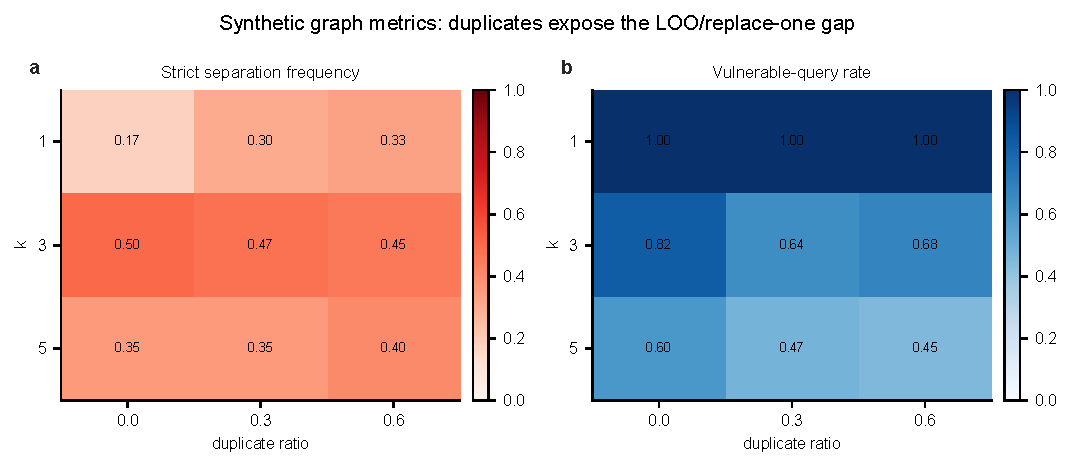
\includegraphics[width=\linewidth]{outputs/figures/fig3_synthetic_results.pdf}
    \caption{Synthetic graph-metric benchmark.  The left panel reports the
    frequency of samples that are LOO-stable but replace-one-unstable; the right
    panel reports the fraction of query points whose signed margin lies within
    the single-replacement vulnerability band.}
    \label{fig:synthetic-results}
\end{figure}

\subsection{UCI tabular data}

We evaluate the same metrics on four UCI datasets: Iris, Wine, Breast Cancer
Wisconsin, and Digits.  Each dataset is converted to binary classification
(class~0 vs.\ the rest) and embedded in a Euclidean metric space.  For each
dataset, we draw seeded subsamples and compute the separation frequency and
vulnerable-query rate.

\Cref{fig:tabular-results} shows that tabular data can exhibit the same gap, but
not uniformly across datasets or neighborhood sizes.  This is the point of the
experiment: LOO failure is not universal, yet it is concrete and detectable
once replace-one vulnerability is measured directly rather than inferred from
LOO behavior.

\begin{figure}[t]
    \centering
    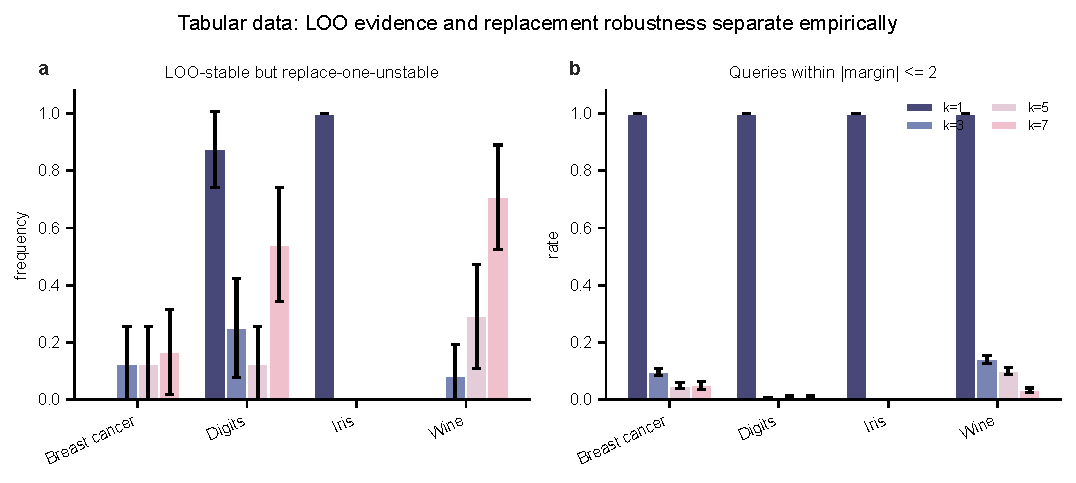
\includegraphics[width=\linewidth]{outputs/figures/fig4_tabular_results.pdf}
    \caption{Tabular benchmark.  Separation frequency and vulnerable-query rate
    are reported across binary tabular datasets and neighborhood sizes.  Error
    bars are the confidence intervals generated by the benchmark pipeline.}
    \label{fig:tabular-results}
\end{figure}

\subsection{Margin-based vulnerability diagnostic}

The margin-based diagnostic ($|\M_k(S,x)| \le 2$ flags a query as potentially
vulnerable) is not merely a heuristic: for odd $k$, a single replacement
alters the ordered vote by at most $\pm 2$, so the margin can cross zero if and
only if $|\M_k(S,x)| \le 2$.  This follows directly from the fact that
replacing one occurrence changes the top-$k$ set by at most two entries, each
contributing $\pm 1$ to the signed margin.  Consequently the diagnostic has
precision and recall identically $1$ on all odd-$k$ configurations---no
empirical validation is needed.  For even $k$ the situation is more complex
because the margin is always even and the $0 \prec 1$ tie-break creates
additional asymmetry.

The practical upshot is that practitioners can efficiently identify potentially
vulnerable queries by computing the margin distribution rather than relying
solely on aggregate LOO error.

\subsection{Empirical summary}

\begin{enumerate}[leftmargin=*,label=(\arabic*)]
    \item The LOO/replace-one separation appears at measurable frequency in
        random graph metrics under controlled duplicate and conflict regimes.
    \item The tabular benchmark shows that the gap is not confined to the
        minimal two-point witness, while also showing that the frequency is
        dataset- and $k$-dependent.
    \item The vulnerable-query rate ($|\M_k| \le 2$) is a reliable diagnostic
        for odd $k$.
    \item The figures should be read as reproducible finite-sample evidence,
        not as distribution-free probability statements.
\end{enumerate}

These findings support the claim that the LOO/replace-one separation is a
structurally stable phenomenon detectable beyond hand-crafted examples.  Full
experimental protocol, parameters, and random seeds are reported in
\Cref{app:experimental-protocol}.
